\documentclass[a4paper,11pt,twoside,pdftex]{article}

% Caption package for formating figure and label captions
\usepackage[font=bf,format=hang,labelsep=colon,justification=justified,singlelinecheck=false,compatibility=false]{caption}


% Misc packages
\usepackage{ifthen} % for conditional expressions
\usepackage{float} % for floating tables and graphics
\usepackage{setspace} % for defining spacing between lines
\usepackage{cmap} % allow searching in pdf documents
\usepackage{tabulary} % better tables
\usepackage{comment} % block comments
\usepackage[T1]{fontenc} % for searching for terms with underscores
\usepackage{listings} % for writing Code
\usepackage{csquotes} % for writing Code
\usepackage[usenames, dvipsnames]{color} % Highlighting text for editing
\usepackage{xcolor}
% hyperref for HTML links within pdf 
%% EXAMPLE: \href{http://www.niwa.co.nz}{NIWA}
\usepackage[bookmarks=true,bookmarksopen=false,bookmarksnumbered=true,
            pdfpagelayout=TwoPageRight,
            pdftitle={Casal2 Contributors Guide}, 
            pdfauthor={C. Marsh} %authors
            pdfsubject={Casal2 Contributors Guide},
            pdftex]{hyperref}
\hypersetup{
  breaklinks=true,      % allow line breaks in URLs
  colorlinks=true,      % use colour to define links
  linkcolor=black,      % colour of internal links
  citecolor=black,      % colour of links to bibliography
  filecolor=black,      % colour of file links
  urlcolor=darkgray     % colour of external links
}
\pdfadjustspacing=1

\definecolor{codegreen}{rgb}{0,0.6,0}
\definecolor{codegray}{rgb}{0.5,0.5,0.5}
\definecolor{codepurple}{rgb}{0.58,0,0.82}
\definecolor{backcolour}{rgb}{0.95,0.95,0.92}

\lstdefinestyle{Rstyle}{
	backgroundcolor=\color{backcolour},   
	commentstyle=\color{codegreen},
	keywordstyle=\color{magenta},
	numberstyle=\tiny\color{codegray},
	stringstyle=\color{codepurple},
	basicstyle=\ttfamily\footnotesize,
	breakatwhitespace=false,         
	breaklines=true,                 
	captionpos=b,                    
	keepspaces=true,                 
	numbers=left,                    
	numbersep=5pt,                  
	showspaces=false,                
	showstringspaces=false,
	showtabs=false,                  
	tabsize=2
}
\lstset{style=Rstyle}
% Use AMS Maths 
\usepackage[fleqn]{amsmath}
\newcommand\AddVspace{\\[0 pt]} % artificial method of adding vertical space within equations

% Package for including and pretty printing of external config files and program code
\usepackage{listings} 
\lstset{ %
basicstyle=\ttfamily\footnotesize,
breaklines=true,
columns=fullflexible,
showspaces=false,               % show spaces adding particular underscores
showstringspaces=false,         % underline spaces within strings
showtabs=false,                 % show tabs within strings adding particular underscores
tabsize=2,			            % sets default tabsize to 2 spaces
breakatwhitespace=false,	    % sets if automatic breaks should only happen at whitespace
escapeinside={\%*}{*)}          % if you want to add a comment within your code
}

% highlighting package for editing
\usepackage{color,soul}

% Allow colour for HTML links
\usepackage{color}
\definecolor{darkgray}{gray}{0.20}
\definecolor{lightgray}{gray}{0.95}

% Geometery for A4 layout like MS-Word defaults
\usepackage[left=2.54cm,top=2.54cm,bottom=3.17cm,right=3.17cm]{geometry}

% Natlib to better cite references (round brackets, commas between refs, and sorted)
\usepackage[round,comma,sort]{natbib}

% Making the index
\usepackage{makeidx}
\makeindex

% Graphics (no postscript files.. just use jpeg, png, etc)
\usepackage[dvips]{graphicx}
% Changes fonts to Times, Helvetica, Courier
\usepackage{pslatex} 

% Section header fonts
\usepackage{sectsty}
\allsectionsfont{\sffamily\large} % Normal sized arial style section headings
% Add a dot after section headings
\makeatletter
 \def\@seccntformat#1{\csname the#1\endcsname.\quad}
 \renewcommand\paragraph{\@startsection{paragraph}{4}{\z@}%
             {-2.5ex\@plus -1ex \@minus -.25ex}%
             {1.25ex \@plus .25ex}%
             {\normalfont\normalsize\bfseries}}
\makeatother

\setcounter{secnumdepth}{4} % how many sectioning levels to assign numbers to
\setcounter{tocdepth}{4}    % how many sectioning levels to show in ToC

% Page style
\usepackage{fancyhdr}
\pagestyle{fancy}
\fancyhead{}
\fancyfoot{}
\headheight 15pt
\renewcommand{\headrulewidth}{0pt} % rule line under header
\renewcommand{\footrulewidth}{0pt}
\setlength{\parindent}{0pt} % No indentation at start of paragraph
\setlength{\baselineskip}{1ex plus 0.2ex minus 0.1ex}
\setlength{\parskip}{1.1ex} % Gap between paragraphs
\raggedbottom % prefer space at the bottom of page
						
% Make equation numbers be section number then equation number
\makeatletter
\@addtoreset{equation}{section}
\@addtoreset{figure}{section}
\@addtoreset{table}{section}
\def\thefigure{\thesection.\@arabic\c@figure}
\def\thetable{\thesection.\@arabic\c@table}
\def\theequation{\thesection.\@arabic\c@equation}
\makeatother

%% stop figures from going onto a page by themselves 
\renewcommand{\topfraction}{0.85}
\renewcommand{\textfraction}{0.1}
\renewcommand{\floatpagefraction}{0.75}

% Minimise hyphen use
\hyphenpenalty=5000
\tolerance=1000

% Compact titles
%\usepackage[small,compact]{titlesec} 

% New commands to define macros and other aids to text and layout
\newcommand{\config}{input configuration file}
\newcommand{\command}[1] {\texttt{@#1}}
\newcommand{\subcommand}[1] {\texttt{#1}}
\newcommand{\commandsub}[2] {\command{#1}\subcommand{.#2}}
\newcommand{\commandlabsub}[2] {\command{#1\texttt{[label]}}\subcommand{.#2}}
\newcommand{\argument}[1] {\texttt{#1}}
\newcommand{\commandsubarg}[3] {\command{#1}\subcommand{.#2}\argument{=#3}}
\newcommand{\commandlabsubarg}[3] {\command{#1\texttt{[label]}}\subcommand{.#2}\argument{=#3}}

\newcommand{\commentline}{\#}
\newcommand{\commentstart}{\{}
\newcommand{\commentend}{\}}

\newcommand{\textlow}[1]{\raisebox{-.4ex}{\scriptsize #1}}

% command shortcuts:
\newcommand{\Rzero}{\emph{R}$_0$}
\newcommand{\Bzero}{\emph{B}$_0$}
\newcommand{\R}{\textbf{R}}
\newcommand{\SSBoff}{$SSB_{\text{offset}}$}

%quick index:
\newcommand{\I}[1]{#1\index{#1}}

% New commands to template syntax definitions: copied from SPM, setup needs defining
% Define a command without a label
\newcommand{\defCom}[2]{\texttt{\textbf{@#1}\index{Command ! #1}} \hspace{0.5cm} {#2}}
% Define a command with a label
\newcommand{\defComLab}[2]{\texttt{\textbf{@#1}\ \emph{label}\index{Command ! #1}} \hspace{0.5cm} {#2}}
% Define a subcommand
\newcommand{\defSub}[2]{\texttt{#1} \hspace{0.5cm} #2 \\*}% Define a command with an argument
\newcommand{\defComArg}[3]{\texttt{\textbf{@#1}\ \emph{#2}\index{Command ! #1}} \hspace{0.5cm} {#3}}
% Define a Command\index{Command} argument
\newcommand{\defArg}[2]{\emph{\texttt{#1}} \hspace{0.5cm} #2 \\*}

% Generic definition for subcommand syntax: copied from SPM, setup needs defining
\newcommand{\defText}[2]{\hangindent=0.3cm \small{#1\ #2}\normalsize \\*}
% Define subcommand syntax for Type / Default / Condition / Value / Note / Example / Lower Bound / Upper Bound
\newcommand{\defType}[1]{\defText{Type:}{#1}}
\newcommand{\defDefault}[1]{\defText{Default:}{#1}}
\newcommand{\defCondition}[1]{\defText{Condition:}{#1}}
\newcommand{\defValue}[1]{\defText{Value:}{#1}}
\newcommand{\defNote}[1]{\defText{Note:}{#1}}
\newcommand{\defExample}[1]{\defText{Example:}{#1}}
\newcommand{\defLowerBound}[1]{\defText{Lower Bound:}{#1}}
\newcommand{\defUpperBound}[1]{\defText{Upper Bound:}{#1}}
\newcommand{\defAllowedValues}[1]{\defText{Allowed Values:}{#1}}

% Input CASAL2 version definitions
% WARNING: THIS FILE IS AUTOMATICALLY GENERATED BY doBuild version. DO NOT EDIT THIS FILE
\newcommand{\Version}{22.09 (2022-09-02)}
\newcommand{\VersionNumber}{22.09}
\newcommand{\SourceControlRevision}{218948c033623d021dd341b8df4c1e7866adfef8}
\newcommand{\SourceControlDateDoc}{2022-09-02}
\newcommand{\SourceControlYearDoc}{2022}
\newcommand{\SourceControlMonthDoc}{September}
\newcommand{\SourceControlTimeDoc}{00:23:03}
\newcommand{\SourceControlVersion}{2022-09-02 00:23:03 UTC (rev. 218948c)}

\newcommand{\DocYear}{\SourceControlYearDoc}
\newcommand{\DocMonth}{\SourceControlMonthDoc}
\newcommand{\DocDate}{\SourceControlMonthDoc\ \SourceControlYearDoc}
\newcommand{\DocVer}{\SourceControlDateDoc}

%New commands to automate document dates, manual titles, document reference, etc.
\newcommand{\VER}{v\SourceControlDateDoc} % CASAL2 program version
\newcommand{\CNAME}{Casal2}
\newcommand{\cname}{\texttt{casal2}} % casal2 binary name
\newcommand{\authors}{C. Marsh and S. Rasmussen}
\newcommand{\email}{casal2@niwa.co.nz}
\newcommand{\github}{\url{https://github.com/NIWAFisheriesModelling/CASAL2}}
\newcommand{\authorlink}{\href{mailto:"CASAL2 Development Team"<casal2@niwa.co.nz>?subject=Casal2:}{authors}} 
%hyper ref for email
\newcommand{\Organisation}{National Institute of Water \& Atmospheric Research Ltd.}
\newcommand{\ManualRef}{\authors\ (\DocYear). \CNAME\ Contributors Guide, \VER. \ref{TotPages} p. (Using source code from \SourceRepos)} % full document reference

% Define \clearemptydoublepage so-as to have truly blank pages between sections
\let\origdoublepage\cleardoublepage
\newcommand{\clearemptydoublepage}{%
  \clearpage
  {\pagestyle{empty}\origdoublepage}%
}
%% Commands for the license section taken from http://www.gnu.org/licenses/lgpl-3.0.tex
\renewcommand{\labelenumii}{\alph{enumii})}
\renewcommand{\labelenumiii}{\arabic{enumiii})}

% Load package to count the number of pages in document
% For getting number of pages in document (NOT the last page number printed), use \ref{TotPages}
% Load this last to ensure its macros are not overwritten
\usepackage{totpages} 

\makeatother

%Begin the document
\begin{document} 
\hbadness=10000 % to deal with underfull hbox warnings
\sloppy % use sloppy paras

% Title page
\pdfbookmark[1]{Casal2 Contributors Guide}{title}
\pagenumbering{alph} % alpha not used, but used to remove warnings when page 1 is re-defined below

\begin{titlepage}
  \thispagestyle{empty} % no header/footer/page number on this page
	\begin{center}

		\vspace*{2.5cm}
		\Huge \CNAME\ Contributors Guide \\

		\vspace{2.0cm}
		\huge \authors \\ %Document authors

		\vspace{2cm}
		\begin{figure}[htp]
			\begin{center}
			
\includegraphics[height=7cm]{Figures/CASAL2.png}
			\end{center}
		\end{figure}

		~\vfill
%		\Large NIWA Technical Report 139 \\%Document Date
%		\Large ISSN 1174-2631 \\%Document Date
%		\Large \DocYear \\%Document Date

		\Large
		\vspace{1.0cm}
		\CNAME\ Contributors Guide for use with \CNAME~(\VER) \\ \SourceRepos
	
	\end{center}
\end{titlepage}


% Citation page
% Citation page
%\cleardoublepage{}
%\fancyfoot[C]{\thepage}
%\pagenumbering{roman}

~\vfill

\begin{center}
Citation: \ManualRef    
\end{center}

% Table of contents
\clearemptydoublepage{}
\pdfbookmark[1]{Contents}{contents}

\begin{spacing}{0.8} % Reduce space between lines in contents list
\tableofcontents
\end{spacing}

% Table of figures
%\clearemptydoublepage{}
%\pdfbookmark[1]{List of figures}{figures}
%\begin{spacing}{0.8} % Reduce space between lines in contents list
%\renewcommand\listfigurename{List of figures}
%\listoffigures
%\end{spacing}

% Table of tables
%\clearemptydoublepage{}
%\pdfbookmark[1]{List of tables}{tables}
%\begin{spacing}{0.8} % Reduce space between lines in contents list
%\renewcommand\listtablename{List of tables}
%\listoftables
%\end{spacing}

% Document body
\clearemptydoublepage{}
\renewcommand{\headrulewidth}{0.2pt}
\fancyhead[RO]{\slshape \nouppercase \rightmark} % Section headings at top of page (header, odd pages)
\fancyhead[LE]{\slshape \nouppercase \leftmark}  % Section headings at top of page (header, even pages)
\pagenumbering{arabic} % Page numbers a arabic numerals

%\include{equations}

\section{Introduction}\label{sec:introduction}

This document is a help guide for \CNAME\, age-structured population modelling software package. This short document is aimed at users who are new to \CNAME. As the names suggests \CNAME\ is a generalised tool for carrying out age-structured population dynamics models, including fisheries assessments and other population dynamics problems. 

\CNAME is very generalised, highly flexible, and therefore can be a bit daunting at first sight. It has a large number of run modes, settings, and user defined population dynamics choices that can turned on and off, depending on the circumstances and the user requirements. While there is no requirement for a user to see or understand the underlying code base, it has been written so that is is well tested and great effort has been put into developing a code base that can be easily interpreted and understood by even novice programmers

\CNAME is open source, and is covered under the GNU GPL 2.0 licence. See the terms and conditions in the user manual \citep{CASAL2}, or type \texttt{casal2 -v} into the command prompt. There is also supplementary information that may be useful to have access while reading this. This includes a more comprehensive and detailed user manual which goes into \CNAME\ in more depth. 

Also coming soon will be a document on how \CNAME\ has inbuilt testing of code, and another validation document comparing \CNAME\ predecessor with \CNAME\. These can all be found in \CNAME\ file that is installed with the installer. By this stage we are assuming you have installed \CNAME\ using the \texttt{casal2\_setup.exe}. This will install \CNAME\ into your path and create a folder in a location of your choice containing, source code, examples, a manual, an R library, this document, an executable and auxiliary libraries.


\section{Creating a local repository\label{sec:local_repo}}

This section will cover the following points

\begin{enumerate}
	\item Registering a github username
	\item Download git software
	\item Fork the master repository
\end{enumerate}

\subsection{Git Username and Profile}

The first step is to create a username and profile on github (if you do not already have one). Creating a username and profile on github is free and easy to do. 

Go to \url{https://www,github.com} to register a username and set up a profile if you do not already have one. See the help at github for more information. Once you have set up a github account you need download the git software that you use to ``communicate" with repositories (places where the software source code is stored) on github.

\subsection{Git Software}

You will need to acquire a git client in order to clone a copy of the source code and link this to the repository.

\CNAME\ also requires a command line version of git in order to compile. The \CNAME\ build environment requires git in order to evaluate the version of the code used at compile time to include into the executable and manual when being built. 

One package that allows this on a Microsoft Windows platform is tortoisegit (see \url{https://tortoisegit.org/download}) to pull, push and commit changes to git repositories. However there are many other clients that could be used to achieve the same functionality.

\subsection{Cloning a repository}

The publicly available \CNAME\ code is in the master repository. Only the \CNAME\ Development Team have permission to add, delete, or change code in the master repository. Other contributors can either add, delete, or change code either by forking the master repository' or by maintaining a local version of the repository. Forking a copy on github can be done at \url{https://github.com/NIWAFisheriesModelling/CASAL2} by selecting the fork button in the top right of the page circled in Figure~\ref{fig:fork}

\begin{figure}[!ht]
	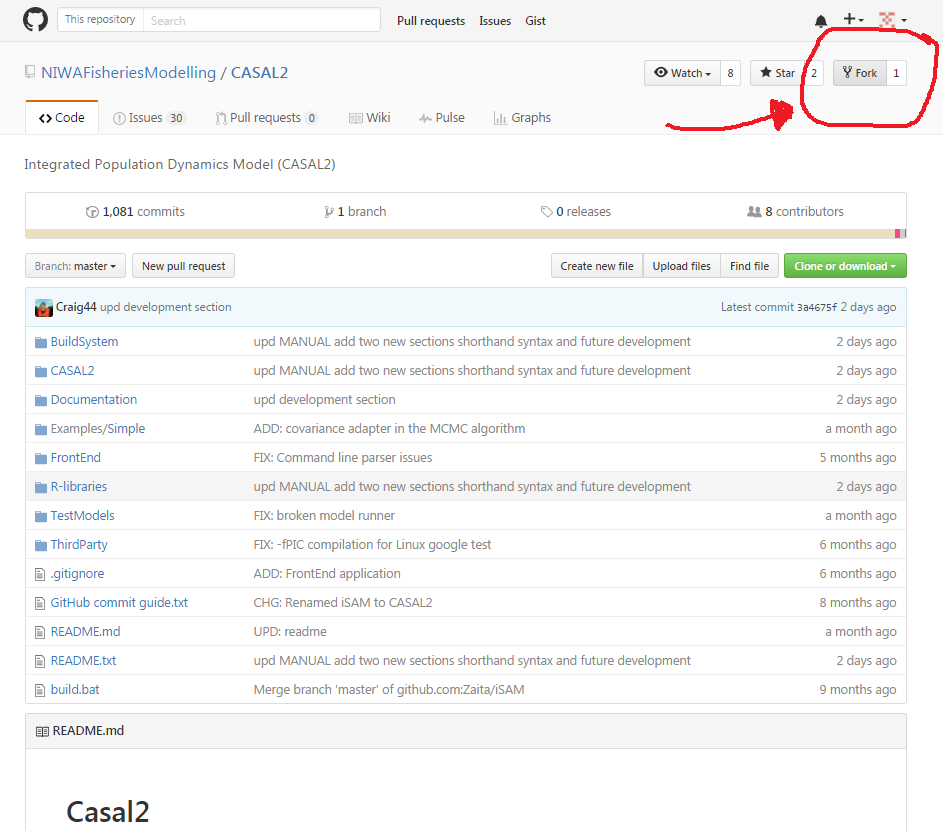
\includegraphics[scale=0.6]{Figures/Fork_button.png}
	\caption{Creating a forked repository}\label{fig:fork}
\end{figure}
\pagebreak

This will create a copy of the \CNAME\ repository under your profile at the point of the fork. To check that you have successfully forked the repository, go to your git profile and you should see a \CNAME\ repository under your repositories, shown in Figure~\ref{fig:fork_success},

\begin{figure}[!ht]
	\includegraphics[scale=0.6]{Figures/Fork_success.png}
	\caption{Fork success}\label{fig:fork_success}
\end{figure}

An important point is that the forked repository will not automatically keep up to date with the master repository. So if the master changes, you will want to keep your forked repository up to date. This can easily be done and is explained in the next section.


 

\section{Create a branch to start making changes\label{sec:maintain_repo}}

This section covers how to create a branch and the importance of the naming convention that is used to track all the development. 

If you are using git client from the command prompt then creating a branch is easy by using the following command \texttt{git -b <BranchLabel>}. The \texttt{BranchLabel} has a specific naming convention, which is  \texttt{BranchLabel \ = \ simpledescription\_YYYYMM}. For example \texttt{git -b SplineSelectivity\_202307} which is adding or fixing the spline selectivity class which started in July of 2023. This makes it easier for the Development Team what is in the branch and how active it is.

Once you have created a branch you can switch between the master and branch using the \texttt{git checkout} command. To find out how to merge changes from the master into your branch just google \enquote{git merging master into feature branch} and you will find many useful resources.

\CNAME\ Once you do your first push to the branch it you will then be able to see it under the branches tab on the online master repository (See Figure~\ref{fig:branchtab}). If you have trouble pushing the branch you may need one of the \CNAME\ developers to add you as a collaborator to the project. This would mean someone has to log into the GitHub account for the repository, go to settings tab, and add the user as a collaborator (left tab panel).

\begin{figure}[!ht]
	\centering
	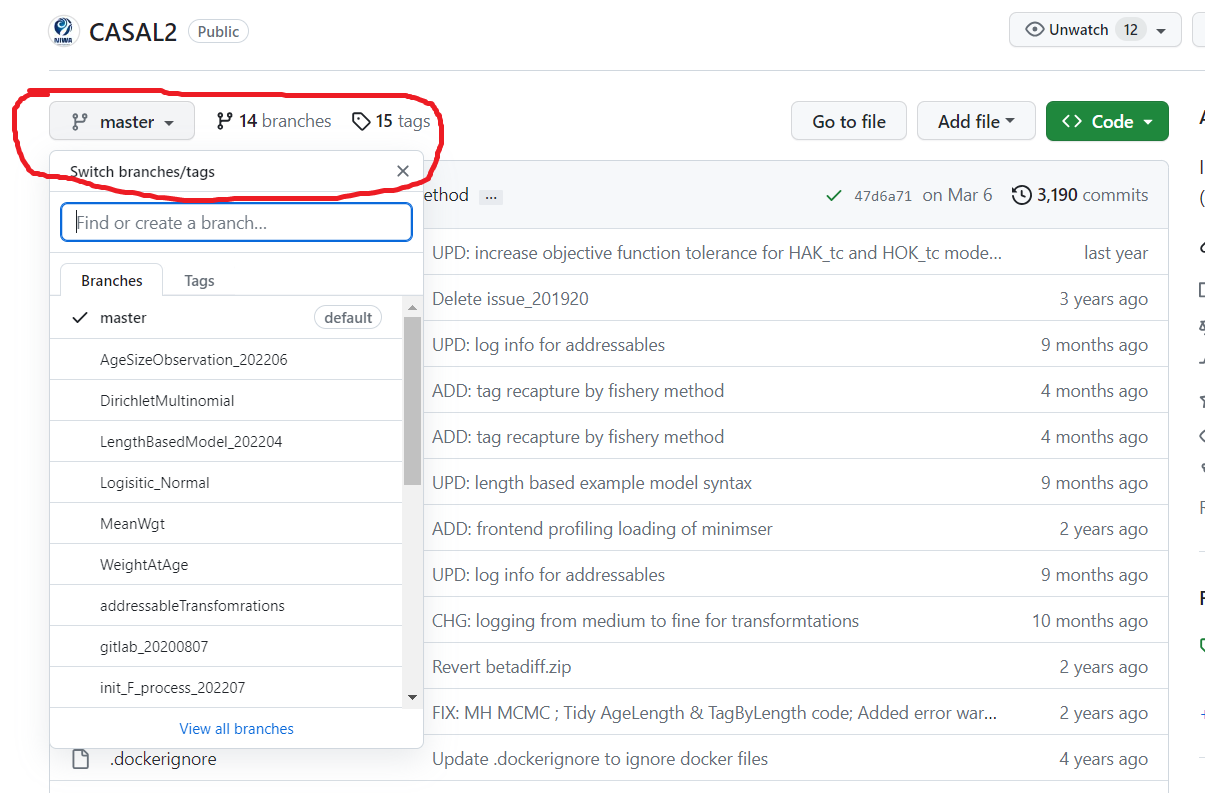
\includegraphics[scale=0.6]{Figures/branch_tab.png}
	\caption{Example of choosing the branch in GitHub}\label{fig:branchtab}
\end{figure}

%\section{Setting up \CNAME\ BuildSystem\label{sec:build_environment}}

This section descibes how to set up the environment on your local machine that will allow you to build and compile \CNAME\. The buld enviroment can be on either Microsoft Windows or Linux systems. At present the \CNAME\ build system supports Microsoft Windows 7+ and Linux (with GCC/G++ 4.9.0+). Apple OSX or other platforms are not currently supported.

\subsection{Overview}

The build system is made up of a collection of python scripts that do various tasks. These are located in \path{CASAL2/BuildSystem/buildtools/classes/}. Each python script has it’s own set of functionality and undertakes one set of actions. 

The top level of the build system can be found at \path{CASAL2/BuildSystem/}. In this directory you can run \texttt{doBuild.bat help} from the command line in Microsoft Windows systems or \texttt{./doBuild.sh help} from a terminal in Linux systems.
 - this doesn't make sense.
The build system will take one or two parameters depending on what style of build you'd like to achieve. These commands allow the building of various stand-alone binaries, shared libraries, and the documentation. Note that you will need additional software installed on your system in order to build \CNAME . These requirements are described later.

A summary of all of the doBuild arguments can be found using the command \texttt{doBuild help} in the BuildSystem directory.

The current arguments to doBuild are: 

\begin{itemize}
  \item \texttt{debug}:  Build standalone debug executable
  \item \texttt{release}: Build standalone release executable
  \item \texttt{test}: Build standalone unit tests executable
  \item \texttt{documentation}: Build the user manual
  \item \texttt{thirdparty}: Build all required third party libraries
  \item \texttt{thirdpartylean}: Build minimal third party libraries
  \item \texttt{clean}: Remove any previous debug/release build information
  \item \texttt{cleanall}: Remove all previous build information
  \item \texttt{archive}: Build a zipped archive of the application. The application is built using shared libraries so a single casal2 executable is created. 
  \item \texttt{check}: Do a check of the build system
  \item \texttt{modelrunner}: Run the test suite of models
  \item \texttt{installer}: Build an installer package
  \item \texttt{deb}: Create Linux .deb installer
  \item \texttt{library}: Build shared library for use by front end application
  \item \texttt{frontend}: Build single CASAL2 executable with all minimisers and unit tests
\end{itemize}

Valid Build Parameters: (thirdparty only)
\begin{itemize}
  \item \texttt{<libary name>}: Target third party library to build or rebuild
\end{itemize}

Valid Build parameters: (debug/release only)
\begin{itemize}
  \item \texttt{betadiff}: Use BetaDiff auto-differentiation (from CASAL)
  \item \texttt{cppad}: Use CppAD auto-differentiation
  \item \texttt{adolc}: Use ADOLC auto-differentiation in compiled executable
\end{itemize}

Valid Build parameters: (library only)
\begin{itemize}
  \item \texttt{adolc}: Build ADOLC auto-differentiation library
  \item \texttt{betadiff}: Build BetaDiff auto-differentiation library (from CASAL)
  \item \texttt{cppad}: Build CppAD auto-differentiation library
  \item \texttt{test}: Build Unit Tests library
  \item \texttt{release}: Build release library
\end{itemize}

The outputs from the build system commands will be placed in subfolders of \path{CASAL2/BuildSystem/bin/<operating system>/<build_type>}

For example:

\path{CASAL2/BuildSystem/windows/debug}

\path{CASAL2/BuildSystem/windows/library_release}

\path{CASAL2/BuildSystem/windows/thirdparty/}

\path{CASAL2/BuildSystem/linux/library_release}

\subsection{Building on Windows}

\subsubsection{Prerequisite Software}

The building of \CNAME\ requires additional build tools and software, including git version control, GCC compiler, LaTex compiler, and an Windows package builder. \CNAME\ requires specific implementations and versions in order to build. 

\textbf{C++ and Fortran Compiler}

Source: tdm-gcc (MingW64) from \url{http://www.tdm-gcc.tdragon.net/}.

\CNAME\ is designed to compile under GCC on Microsoft Windows and Linux  platforms. While it may be possible to build the package using different compilers, the \CNAME\ Development Team does provide any assistance or recommendations. We recommend using 64-bit TDM-GCC version 5.1.0. Ensure you have the "fortran" and "openmp" options installed as a part of the "gcc" dropdown tickboxes otherwise \CNAME will not compile.. \textbf{Note}: A common error that can be made is having a different GCC compiler in your path when attempting to compile. For example, rtools includes a version of the GCC compiler. We recommend removing these from your path prior to compiling.


\textbf{GIT Version Control}

Source: Command line GIT from \url{https://www.git-scm.com/downloads}.

\CNAME\ automatically adds a version number based on the GIT version of the latest commit to its repository. The command line version of GIT is used  to generate a version number for the compiled binaries, R libraries, and the manuals. 

\textbf{MiKTeX Latex Processor}

Source: Portable version from \url{http://www.miktex.org/portable}. 

The main user documentation for \CNAME\ is a PDF manual generated from LaTeX. The LaTeX syntax sections of the documentation are generated, in part, directly from the code. In order to regenerate the user documentation, you will need the MiKTeX LaTeX compiler.

\textbf{7-Zip}

Source: 7-Zip from \url{http://www.7-zip.org/download.html}.
	
The BuildSystem calls 7zip.exe to unzip files in the build system; it is advised to have this in the path.

\textbf{Inno Setup Installer Builder (optional)}

Source: Inno Setup 5 from \url{http://www.jrsoftware.org/isdl.php}

If you wish to build a Microsoft Windowes compatible Installer for \CNAME\ then you will need the Inno Setup 5 application installed on the machine. The installation path must be \path{C:\Program Files (x86)\Inno Setup 5\} in order for the build scipts to fins and use it.

\subsubsection{Pre-Build Requirements}

Prior to building \CNAME\ you will need to ensure you have both G++ and GIT in your path. You can check both of these by typing:

\texttt{g++ --version}

\texttt{git --version}

This also allows you to check that there are no alternative versions of a GCC compiler that may confuse the \CNAME\ build. 

It’s worth checking to ensure GFortran has been installed with the G++ compiler by typing:

\texttt{gfortran --version}

If you wish to build the documentation bibtex will also need to be in the path:

\texttt{bibtex -version}

\subsubsection{Building \CNAME}

The build process is relatively straightforward. You can run \texttt{doBuild check} to see if your build environment is ready.

\begin{enumerate}
  \item Get a copy (clone) of the forked code on your local machine, mentioned in Section~\ref{sec:local_repo}: 
  \item Navigate to the BuildSystem folder in \path{CASAL2/BuildSystem}
  \item You need to build the third party libraries with:
  \begin{itemize}
    \item \texttt{doBuild thirdparty}
  \end{itemize}
  \item You need to build the binary you want to use:
  \begin{itemize}
    \item \texttt{doBuild release}
  \end{itemize}	
  \item You can build the documentation if you want:
  \begin{itemize}
    \item \texttt{doBuild documentation}
  \end{itemize}		
\end{enumerate}

\subsection{Building on Linux}

This guide has been written against a fresh install of Ubuntu 15.10. With Ubuntu we use apt-get to install new packages. You’ll need to be familiar with the package manager for your distribution to correctly install the required prerequisite software.

\subsubsection{Prerequisite Software}

\textbf{Compiler G++}

Ubuntu 15.10 comes with G++ 15.10, gfortran is not installed though so we can install it with: \texttt{sudo apt-get install gfortran}.

\textbf{GIT Version Control}

Git isn't installed by default but we can install it with \texttt{sudo apt-get install git}

\CNAME\ automatically adds a version number based on the GIT version of the latest commit to its repository. The command line version of GIT is used  to generate a version number for the compiled binaries, R libraries, and the manuals. 

\textbf{CMake}

CMake is required to build multiple third-party libraries and the main code base. You can do this with \texttt{sudo apt-get install cmake}

\textbf{Python2 Modules}

There are a couple of Python2 modules that are required to build \CNAME. These can be installed with \texttt{sudo apt-get install python-dateutil}

You may also need to install \textbf{datetime}, re and \textbf{distutils}. \textbf{Texlive} Latex Processor. No supported latex processors are installed with Ubuntu by default. You can install a suitable latex process with:

\texttt{sudo apt-get install texlive-binaries}
\texttt{sudo apt-get install texlive-latex-base}
\texttt{sudo apt-get install texlive-latex-recommended}
\texttt{sudo apt-get install texlive-latex-extra}

Alternatively you can install the complete package:
\texttt{sudo apt-get install texlive-full}

\subsubsection{Building \CNAME}

The build process is relatively straighforward. You can run \texttt{./doBuild.sh check} to see if your build environment is ready.

\begin{enumerate}
	\item Get a copy (clone) of the forked code on your local machine, mentioned in Section~\ref{sec:local_repo}: 
	\item Navigate to the BuildSystem folder in \path{CASAL2/BuildSystem}
	\item You need to build the third party libraries with:
	\begin{itemize}
	    \item \texttt{./doBuild.sh thirdparty}
	\end{itemize}
	\item You need to build the binary you want to use:
	\begin{itemize}
		\item \texttt{./doBuild.sh release}
	\end{itemize}	
	\item You can build the documentation if you want:
	\begin{itemize}
		\item \texttt{./doBuild.sh documentation}
	\end{itemize}		
\end{enumerate}

\subsection{Troubleshooting}

\subsubsection{Third-party Libraries}

It's possible that there will be build errors or issues building the third-party libraries. If you encounter an error, then it’s worth checking the log files. Each third-party build system stores a log of everything it’s doing. The files will be named

\begin{itemize}
	\item casal2\_unzip.log
	\item casal2\_configure.log
	\item casal2\_make.log
	\item casal2\_build.log
	\item \dots etc,.
\end{itemize}

Some of the third-party libraries require very specialised environments for compiling under GCC on Windows. These libraries are packaged with MSYS (MinGW Linux style shell system). The log files for these will be found in \path{ThirdParty/<library name>/msys/1.0/<library name>/}

e.g: \path{ThirdParty/adolc/msys/1.0/adolc/ADOL-C-2.5.2/casal2_make.log}\\
e.g: \path{ThirdParty/boost/boost_1_58_0/casal2_build.log}

\subsubsection{Main Code Base}

If the unmodified code base does not compile, the most likely cause is an issue with the third-party libraries not being built. Ensure they have been built correctly. As they are outside the control of the Development Team, problems can arise that may require the developers of the third party libraries to resolve first. Contact the \CNAME\ development team at \texttt{casal2@niwa.co.nz} for help.




\section{Compiling \CNAME}\label{sec:build_environment}

This section describes how to set up the environment on your local machine that will allow you to build and compile \CNAME. The build environment can be on either Microsoft Windows or Linux systems. At present the \CNAME\ build system supports Microsoft Windows 10+ and Linux (with GCC/G++ 4.9.0+). Apple OSX or other platforms are not currently supported.

\subsection{Overview}

The build system is made up of a collection of python scripts that do various tasks. These are located in \path{CASAL2/BuildSystem/buildtools/classes/}. Each python script has its own set of functionality and undertakes one set of actions.

The top level of the build system can be found at \path{CASAL2/BuildSystem/}. In this directory you can run \texttt{doBuild.bat help} from a command terminal in Microsoft Windows systems or \texttt{./doBuild.sh help} from a terminal in Linux systems.
The script will take one or two parameters depending on what style of build you'd like to achieve. These commands allow the building of various stand-alone binaries, shared libraries, and the documentation. Note that you will need additional software installed on your system in order to build \CNAME .  These requirements are described below.

A summary of all of the doBuild arguments can be found using the command \texttt{doBuild help} in the BuildSystem directory.

The arguments to doBuild are:

Usage: doBuild $<$build\_target$>$ $<$argument$>$
\begin{description}
  \item{help} Print out the doBuild help (this output)
  \item{check} Do a check of the build system
  \item{clean} Remove debug/release build files
  \item{clean\_all} Remove all build files and ALL prebuilt binaries
  \item{version} Build the current version files for C++, R, and LaTeX
\end{description}

Build required libraries (DLLs/shared objects for Casal2)
\begin{description}
  \item{thirdparty} Build the third party libraries
  \begin{description}
    \item{$<$option$>$} Optionally specify the target third party library to build, either adolc or betadiff (default is none)
  \end{description}
\end{description}

Build development and test versions (for development builds only)
\begin{description}
\item{release} Build stand-alone release executable
  \begin{description}
	\item{$<$option$>$} Optionally specify the target third party library to build, either adolc or betadiff (default is none)
  \end{description}
  \item{debug} Build stand-alone debug executable
  \begin{description}
	\item{$<$option$>$} Optionally specify the target third party library to build, either adolc or betadiff (default is none)
  \end{description}
  \item{test} Build stand-alone unit tests executable
  \item{unittests} Run the unit tests
  \item{modelrunner} Run the test suite (requires "test" to have been built)
\end{description}

Build the Casal2 end-user application
\begin{description}
  \item{library} Build shared library for use by front end application
  \begin{description}
    \item{$<$argument$>$} Required argument to specify the target library to build: release, adolc, betadiff, or test
  \end{description}
  \item{frontend} Build \CNAME\ front end application
\end{description}

Create the archive, R Library, documentation, and the installers
\begin{description}
  \item{documentation} Build the \CNAME\ user manuals
  \item{rlibrary} Create the R library
  \item{archive} Create a zipped archive of the \CNAME\ application.
  \begin{description}
     \item{$<$true$>$} if specified build skips everything but frontend
  \end{description}
  \item{installer} Create the Microsoft Windows installer package
  \item{deb} Create Linux .deb installer
\end{description}

The outputs from the build system commands will be placed in sub-folders of \path{CASAL2/BuildSystem/bin/<operating system>/<build_type>}

For example:

\path{CASAL2/BuildSystem/windows/debug}

\path{CASAL2/BuildSystem/windows/library_release}

\path{CASAL2/BuildSystem/windows/thirdparty/}

\path{CASAL2/BuildSystem/linux/library_release}

 The files \texttt{Casal2\_build.bat} for Windows and \texttt{Casal2\_build.sh} for Linux in the root folder contain all the calls in the correct order of \texttt{doBuild} required to successfully build \CNAME, the documentation, the Windows installer (Windows) or the Debian installer (Linux), the R-Libraries, and run all the test cases and unit tests.

\subsection{Building on Windows}

\subsubsection{Prerequisite Software}

The building of \CNAME\ requires additional build tools and software, including git version control, GCC compiler, LaTeX compiler, and a Windows package builder. \CNAME\ requires specific implementations of these packages and versions in order to build without modifying the build scripts.

\textbf{C++ and Fortran Compiler}

Source: tdm-gcc (MinGW-w64) from \url{https://jmeubank.github.io/tdm-gcc/}.

\CNAME\ is designed to compile under GCC on Microsoft Windows and Linux. While it may be possible to build the package using different compilers, the \CNAME\ Development Team does provide any assistance or recommendations. We recommend using 64-bit TDM-GCC with a version of at least 10.3.0. Ensure you have the "fortran" and "openmp" options installed as a part of the "gcc" install option drop-down tick boxes as these are required. For example, from  \url{https://jmeubank.github.io/tdm-gcc/articles/2021-05/10.3.0-release}, select the 64+32-bit MinGW-w64 edition, then select the Custom install and tick all boxes. 

Note that a common error that can be made is having a different GCC compiler in your path when attempting to compile. For example, rtools includes a version of the GCC compiler. We recommend removing these from your path prior to compiling.

\textbf{GIT Version Control}

Source: Command line GIT from \url{https://www.git-scm.com/downloads}.

\CNAME\ automatically adds a version details to its files and any output based on the GIT version of the latest commit to its repository. This includes the name of source repository that was used. The command line version of GIT is used  to generate the version details.

\textbf{MiKTeX Latex Processor}

Source: Portable version from \url{http://www.miktex.org/portable}.

The main user documentation for \CNAME\ is a PDF manual generated from LaTeX. The LaTeX syntax sections of the documentation are generated, in part, directly from the code. In order to regenerate the user documentation, you will need the MiKTeX LaTeX compiler.

\textbf{7-Zip}

Source: 7-Zip from \url{http://www.7-zip.org/download.html}.

The BuildSystem calls 7zip.exe to unzip files in the build system; it is advised to have this in the path.

\textbf{Inno Setup Installer Builder (optional)}

Source: Inno Setup 5 from \url{http://www.jrsoftware.org/isdl.php}

If you wish to build a Microsoft Windows compatible Installer for \CNAME\ then you will need the Inno Setup 5 application installed on the machine. The installation path must be \path{C:\Program Files (x86)\Inno Setup 5\} in order for the build scripts to fins and use it.

\subsubsection{Pre-Build Requirements}

Prior to building \CNAME\ you will need to ensure you have both G++ and GIT in your path. You can check both of these by typing the following commands and checking that they return the correct version number:

\texttt{g++ -{}-version}

\texttt{git -{}-version}

This also allows you to check that there are no alternative versions of a GCC compiler that may confuse the \CNAME\ build. It’s also worth checking to ensure GFortran has been installed with the G++ compiler by typing:

\texttt{gfortran -{}-version}

If you wish to build the documentation bibtex will also need to be in the path, e.g., to check, try:

\texttt{bibtex -{}-version}

\subsubsection{Building \CNAME}

The build process is relatively straightforward. Before you start the build process, you can run \texttt{doBuild check} from the command prompt to check if your build environment is complete. Make sure that you are within \path{CASAL2/BuildSystem/} to run \texttt{doBuild}. 

\texttt{doBuild check} will summarise Windows environment PATH as a part of its output, and this can be used to check that the paths for g++ and gfortran and the g++ point to where the correct version of GCC is installed. 

The build process is as follows: 
\begin{enumerate}
  \item Download a clone of the code on your local machine
  \item Navigate to the BuildSystem folder in \path{CASAL2/BuildSystem}
  \item You need to build the third party libraries with the following commands from the command prompt:
  \begin{itemize}
    \item \texttt{doBuild thirdparty}
  \end{itemize}
  \item You need to build the binary you want to use:
  \begin{itemize}
    \item \texttt{doBuild release}
  \end{itemize}
  \item You can build the documentation if you want:
  \begin{itemize}
    \item \texttt{doBuild documentation}
  \end{itemize}
\end{enumerate}

\subsection{Building on Linux}

This guide has been written against a fresh install of Ubuntu 20.04. With Ubuntu we use apt-get to install new packages. You’ll need to be familiar with the package manager for your distribution to correctly install the required prerequisite software. For this you will require administrator level access.

\subsubsection{Prerequisite Software}

\textbf{Compiler G++}

If gfortran is not installed, install this with: \texttt{sudo apt-get install gfortran}.

\textbf{GIT Version Control}

Git may not be installed by default and it can be installed with \texttt{sudo apt-get install git}

\CNAME\ automatically adds a version details to its files and any output based on the GIT version of the latest commit to its repository. This includes the name of source repository that was used. The command line version of GIT is used  to generate the version details.

\textbf{CMake}

CMake is required to build multiple third-party libraries and the main code base. You can do this with \texttt{sudo apt-get install cmake}

\textbf{Python2 Modules}

There are a number of Python2 modules that are required to build \CNAME. These can be installed with \texttt{sudo apt-get install \texttt{module-name}}. For example, You may need to install \texttt{datetime}, \texttt{re}, and \texttt{distutils} Python modules. 

Latex on Linux is required, and the Texlive Latex Processor is recommended. This can be installed with:

\texttt{sudo apt-get install texlive-binaries}
\texttt{sudo apt-get install texlive-latex-base}
\texttt{sudo apt-get install texlive-latex-recommended}
\texttt{sudo apt-get install texlive-latex-extra}

Alternatively you can install the complete package with 
\texttt{sudo apt-get install texlive-full}

\subsubsection{Building \CNAME}

The build process is relatively straightforward. You can run \texttt{./doBuild.sh check} to see if your build environment is ready.

\begin{enumerate}
	\item Download a clone of the code on your local machine
	\item Navigate to the BuildSystem folder in \path{CASAL2/BuildSystem}
	\item You need to build the third party libraries with:
	\begin{itemize}
	    \item \texttt{./doBuild.sh thirdparty}
	\end{itemize}
	\item You need to build the binary you want to use:
	\begin{itemize}
		\item \texttt{./doBuild.sh release}
	\end{itemize}
	\item You can build the documentation:
	\begin{itemize}
		\item \texttt{./doBuild.sh documentation}
	\end{itemize}
\end{enumerate}

\subsection{Troubleshooting}

\subsubsection{Third-party Libraries}

It's possible that there will be build errors or issues building the third-party libraries. If you encounter an error, then check the log files to locate the source of the problem. Each third-party build system stores a log of everything that was done. The files will be named

\begin{itemize}
	\item casal2\_unzip.log
	\item casal2\_configure.log
	\item casal2\_make.log
	\item casal2\_build.log
	\item \dots etc,.
\end{itemize}

Some of the third-party libraries require very specialised environments for compiling under GCC on Windows. These libraries are packaged with MSYS (MinGW Linux style shell system). The log files for these will be found in \path{ThirdParty/<library name>/msys/1.0/<library name>/}

e.g., \path{ThirdParty/adolc/msys/1.0/adolc/ADOL-C-2.5.2/casal2_make.log}\\
e.g., \path{ThirdParty/boost/boost_1_58_0/casal2_build.log}

A common issue when running doBuild thirdparty are Python error messages about missing modules, e.g., ModuleNotFoundError: No module named 'dateutil'. This type of error message indicates that a Python module (library) is missing and will need to be installed. For instance, to install the 'dateutil' module, type the following into a command prompt or terminal window: pip3 install python-dateutil.  

\subsubsection{Main Code Base}

If the unmodified code base does not compile, the most likely cause is an issue with the third-party libraries not being built correctly. As updates and revisions are outside the control of the Development Team, problems can arise that may require the developers of the third party libraries to resolve first. However, versions of these libraries are included in the \CNAME\ source code and these should work. For any specific issues contact a local expert with regard to your specific system environment, or else the \CNAME\ development team for help.




\clearpage{}

\section{\CNAME\ build guidelines and validation\label{sec:buildrules}}

\subsection{\CNAME\ coding practice and style}\label{subsec:codepractice}

\CNAME\ is written in C++ and uses the Google C++ style guide (see \url{https://google.github.io/styleguide/cppguide.html}). 

In general when editing or writing code for \CNAME\:

\begin{enumerate}
  \item Using consistent indentations inside functions and loops, and descriptive and human readable variable or function names.
  \item Use of the characters `\_' on the end of class variables defined in the .h files. 
  \item Annotate and comment the code, especially where it would help another contributor understand the program logic and rationale.
  \item Add descriptive log messages to aid in debugging and checking of the program logic flow.
  \item Implement unit tests, internal models, and external models to test and validate the new or changed functionality.
  \item Document the functionality in the \CNAME\ User Manual(s).
\end{enumerate}

\CNAME\ allows printing of logging messages art runtime using the --loglevel command line argument. The levels of logging in \CNAME\ are:

\begin{itemize}
	\item LOG\_MEDIUM()  usually reserved for iterative functionality (e.g. estimates during estimation phase)
	\item LOG\_FINE() the level of reporting between an actual report and a fine scale detail that end users are not interested in (Developers)
	\item LOG\_FINEST() Minor fine scale details within a function or routine.
	\item LOG\_TRACE() put at the beginning of every function
\end{itemize}

e.g., to run \CNAME\ with logging, use 

\texttt{casal2 -r --loglevel finest > my\_run.log 2> my\_run.err}

This will output all the logged information to \texttt{my\_run.err}.

\subsection{Units tests and model validation}

The \CNAME\ development places an emphasis on maintaining software integrity and reproducibility between revisions. \CNAME\ uses model validations and built in unit tests to validate and verify the code each time \CNAME\ is compiled and built. 

There are three different validation approaches in \CNAME. These are:

\begin{enumerate}
	\item Mocking specific classes.
	\item Implementing internal models (implemented in C++ source code with extension \texttt{.Test.cpp}) that have variable test cases for specific classes. 
	\item Implementing externally run models (found in the TestModel folder) that are validated to generate expected output.
\end{enumerate}

To implement mocking of classes and internal models, \CNAME\ uses the Google testing framework and the Google mocking framework.

To implement testing of full models, input configuration files are run using the compiled \CNAME\ binaries, and the output compared with expected output using @assert commands.

\subsubsection{Mocking specific classes}

Classes are unit tested using unit tests that are a part of the source code. These are designed to check the components of the code to validate that functions provide expected output. These unit tests are run each time \CNAME\ is compiled.

When adding unit tests, they should to be developed and tested outside of \CNAME\. This gives confidence that the test does not contain any calculation errors. 

Mocking specific classes is used to validate specific functionality and is encouraged because it is the easiest to isolate simple errors that may be introduced with code changes. 

As examples, see (i) the file \texttt{VonBertalanffy.Test.cpp} mocks the von Bertalanffy age-length class and tests the mean length calculation, and (ii) the \texttt{Partition} class has the file \texttt{Partition.Test.cpp} that validates user inputs and model expectations.

\subsubsection{Internal mocking of simple models}

Mocking of simple models is done using a number of internal models. Most of the functionality for implementing these are in the source folder \texttt{/CASAL2/source/TestResources}. 

These implements simple models and run test cases with differing class implementations by running an internal empty model and testing the output of classes from a model run. 

As examples, see (i) the \texttt{LogNormal.Test.cpp} in the \texttt{Projects} class that test the lognormal distribution when used for projections, and (ii) the \texttt{TagByLength} process in \texttt{TagByLength.Test.cpp} that tests functionality of the tagging process.

\subsubsection{External testing using test models}

External tests are run following compilation using the Python modelrunner.py scripts (i.e., using the \texttt{DoBuild modelrunner} script in the BuildSystem folder). These models are used to test model runs, minimisation routines, and MCMC output.

The test model input configuration files are located in the \texttt{TestModel} folder and the command calls to run these are in the modelrunner.py script.  

Contributors are encouraged to add additional models to the list of test models as these be used to validate the combined functionality of a range of interrelated commands and subcommands in \CNAME. 

\subsection{Verification}
After \CNAME\ executes Validate and Build it runs sanity checks in the verify state. These are business rules that can be checked across the entire system. This can be useful to suggest dependencies or configurations. For an example see the directory \subcommand{Processes\textbackslash Verification\textbackslash} in the source code. 

\subsection{Reporting (optional)}

Currently \CNAME\ has reports that are \R\ compatible, i.e., all output reports produced by \CNAME\ can be read into \R\ using the standard  \textbf{CASAL2} \R\ package. If you create a new report or modify an old one, you most follow the standard so that the report is \R\ compatible.

All reports must start with,
\texttt{*label (type)}
and end with,
\texttt{*end}

Depending on what type of information you wish to report, will depend on the syntax you need to use. For example

\paragraph*{$\{$d$\}$ (Dataframe)}
Report a dataframe
{\small{\begin{verbatim}
			*estimates (estimate_value)
			values {d}
			process[Recruitment_BOP].r0 process[Recruitment_ENLD].r0 
			2e+006 8e+006
			*end
\end{verbatim}}}

\paragraph*{$\{$m$\}$ (Matrix)}
Report a matrix
{\small{\begin{verbatim}
			*covar (covariance_matrix)
			Covariance_Matrix {m}
			2.29729e+010 -742.276 -70160.5
			-110126 -424507 -81300 
			-36283.4 955920 -52736.2 
			*end
\end{verbatim}}}

\paragraph*{$\{$L$\}$ (List)}
Report a List
{\small{\begin{verbatim}
			*weight_one (partition_mean_weight)
			year: 1900
			ENLD.EN.notag {L}
			mean_weights {L}
			0.0476604 0.111575 0.199705
			end {L}
			age_lengths {L}
			12.0314 16.2808 20.0135
			end {L}
			end {L}
			*end
\end{verbatim}}}

\subsection{Update the \CNAME\ User Manual(s)}

Contributors will need to add or modify sections of the user manual(s) to document their changes. This includes the section that describes the methods and the section where the specific syntax is defined. 

\subsection{Builds to pass before merging changes}

Once you have made changes, you must run the following before your changes can be included in the master code. 

\begin{itemize}
	\item Build the unittest version. See Section~\ref{sec:build_environment} for how to build unittest depending on your system.
	\item Run the standard and new unit tests to check that they all pass. To do this first compile the test executable using the script \texttt{DoBuild test}. Then move to the directory with the location of the executable (\texttt{BuildSystem/bin/OS/test}) and run it (open a command terminal and run \texttt{casal2}) to check all the unit-tests pass.
	\item Test that the debug and release of \CNAME\ compiles and runs with \texttt{DoBuild debug}
	\item Run the second phase of unit tests (requires that the debug version is built). This runs the tests that comprise of complete model runs using \texttt{DoBuild modelrunner}
	\item Build the archive using \texttt{DoBuild archive} which builds all required libraries. There are small nuances between Double classes, especially when reporting the class that mean seemingly simple changes can sometimes cause a break in the full build.
\end{itemize}




\section{Adding Functionality into \CNAME\label{sec:example}}

The following shows a sequence of figures and text of an example, where we demonstrate how to modify the code base by adding a new child process called SurvivalConstantRate. Although we will be showing adding new process functionality for a process we will explain it in a generalised way so that this can be translated into adding a new selectivity, observation, likelihood, Projection, MCMC, minimiser, time varying class etc.

To add a new process you start by going into the \path{CASAL2\CASAL2\source\processes\}. 
	
	
	\begin{figure}[!ht]
		\centering
		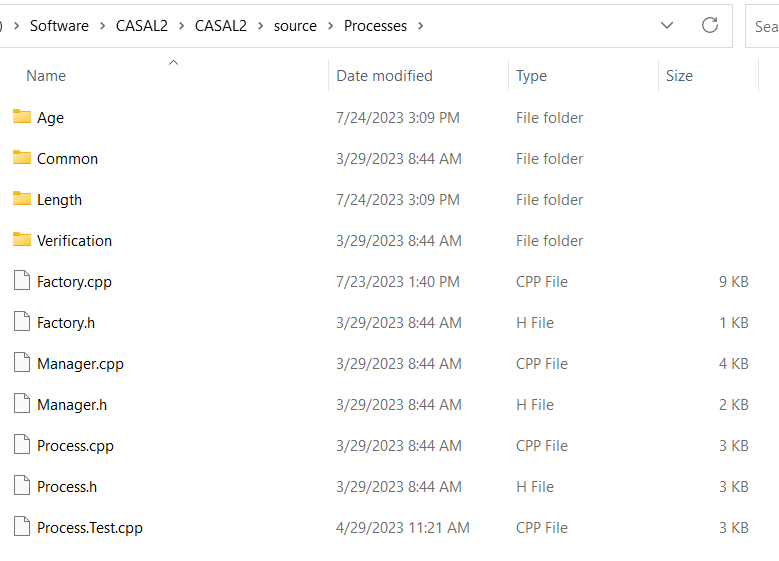
\includegraphics[scale=0.6]{Figures/adding_process1.png}
		\caption{}\label{fig:process}
	\end{figure}


This folder shown in Figure~\ref{fig:process} contains a general layout of all main classes in \CNAME. It contains a folder named \texttt{Children}, C++ source code \texttt{Factory.cpp}, \texttt{Factory.h}, \texttt{Manager.cpp}, \texttt{Manager.h}, \texttt{Process.cpp}, \texttt{Process.h}. The folder \texttt{Children} contains all the current processes implemented in \CNAME. The \texttt{Factory} source code creates all the processes during runtime. The \texttt{Manager} source code manages the class; it can build pointers to specific processes to share information across classes. The \texttt{Process} source code contains base functionality that is inherited by all child classes (inheritance is a major concept in C++ and it is  advised have some knowledge of the concept). Before creating a new child look at the parent (in this example \texttt{Process.cpp}, \texttt{Process.h}), to see the functionality you don't have to add in your child because it is already done at the parent level. The following figure shows the constructor in \texttt{Process.cpp}.
\clearpage
\begin{figure}[!ht]
	\centering
	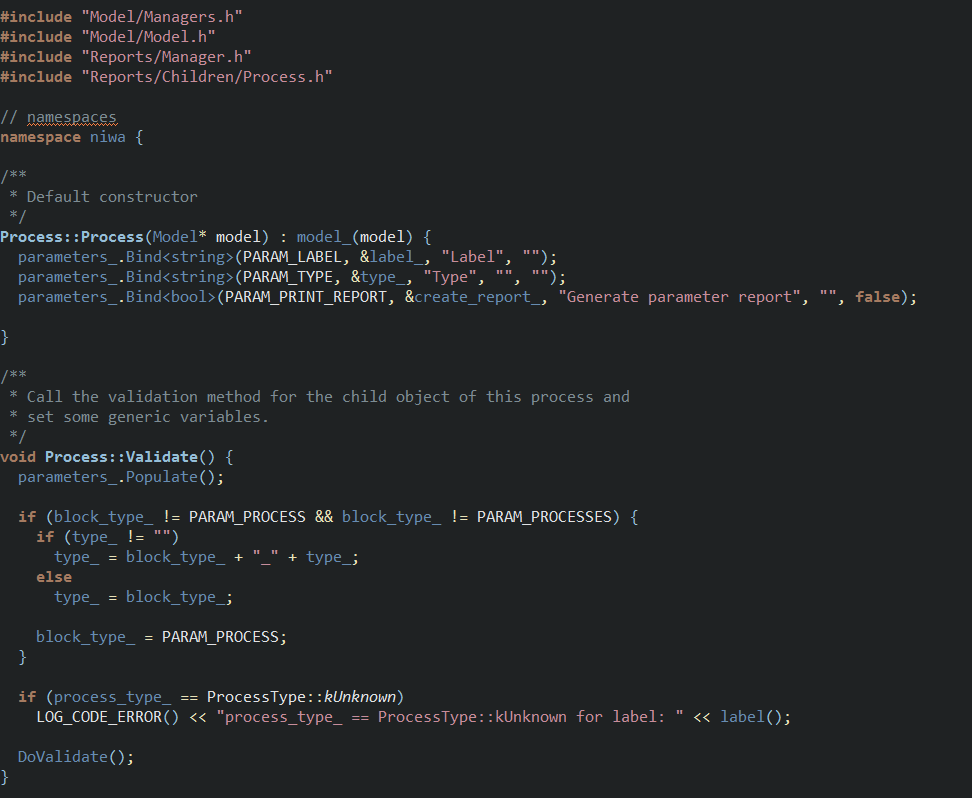
\includegraphics[scale=0.6]{Figures/add_survival1.png}
	\caption{}\label{fig:process1}
\end{figure}

From Figure~\ref{fig:process1} the process parent class does not do much {\color{red}-} it assigns a label and type for each child that will be created and a report subcommand. The point of this is to look at the parent class to reduce duplicating functionality in the child class.


We will be returning to the factory source code later, but for now let's get adding a new process. Enter the \texttt{Children} folder and create C++ source code labelled \texttt{SurvivalConstantRate.cpp} and \texttt{SurvivalConstantRate.h}. These files were should exist in the source code, but fell free to delete them and go through the process of adding the process to see how easy this process is. I usually copy an existing process and rename it, although this is not good coding practice. It's one of those do-as-I-say-not-as-I-do types of things.
\begin{figure}[!ht]
	\centering
	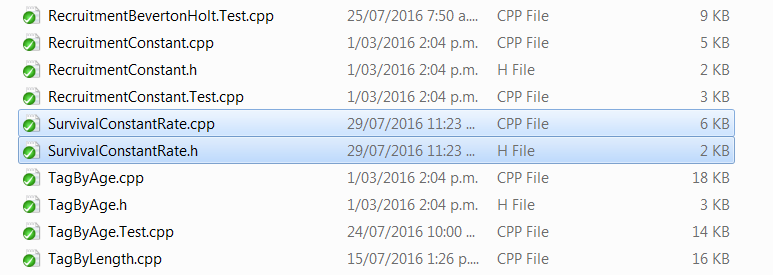
\includegraphics[scale=0.6]{Figures/add_survival.png}
	\caption{}\label{fig:process2}
\end{figure}

Once you have done that for each child class you may have to write code for the following functions{\color{red}:} \texttt{DoValidate()}, \texttt{DoBuild()}, \texttt{PreExecute()}, \texttt{DoExecute()}, \texttt{PostExecute()}, \texttt{DoReset()}. To understand what these all do Figure~\ref{fig:flow} shows the state transition of \CNAME.
\raggedbottom
\begin{figure}[!ht]
	\centering
	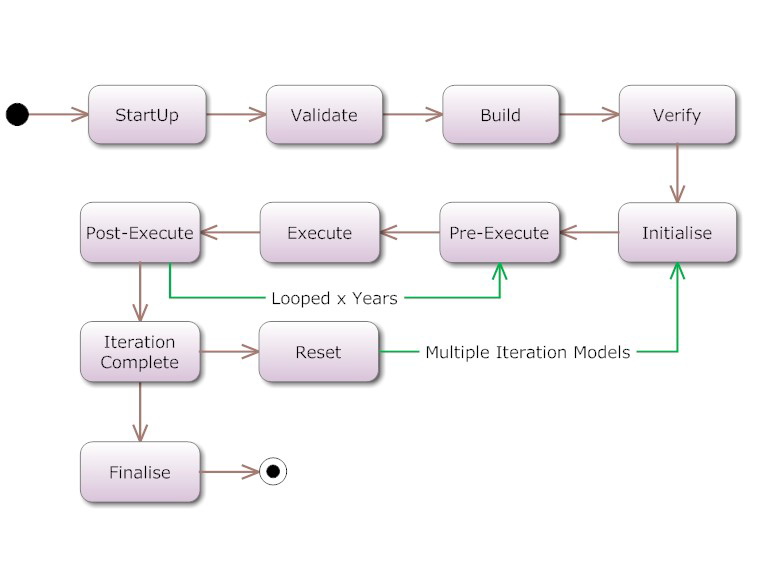
\includegraphics[scale=0.6]{Figures/State-Transition.png}
	\caption{}\label{fig:flow}
\end{figure}

Now we describe the purpose of each transition and this will give you an idea of what you should be incorporating into each function.

\paragraph*{StartUp}
The model is in the blank start and the configuration system is loading the configuration files and parsing any extra inputs.
\\
Tasks completed:
\begin{itemize}
	\item Parse command line
	\item Parse configuration file
	\item Load plugins
	\item Load estimate values from input files
\end{itemize}

\paragraph*{Validate}
All user configurations have been loaded at this point. Now the model will go through every object that has been created and check that the parameters given to them.
\\\\
This step will ensure every object in the model has sufficient parameters to be executed without causing a system fault or error in the model.
\\\\
This state will not check the values to ensure they are logical in relation to an actual model. They will only test that they exist and meet minimum requirements to execute a model.
\\\\
At the end of the validate stage each object should be internally consistent. No lookups or external references are allowed to be formed during this stage.

\paragraph*{Build}
The build phase is where the system will build relationships between objects that rely on each other. Because validation has been completed, each object in it's self-contained configuration is ok.
\\\\
This phase generally assigns values to pointers for objects so they don't need to do lookups of objects during execution phases.

\paragraph*{Verify}
At this point pre-defined configurations are checked against the model's current configuration to verify if the model makes sense logically. These are business rules being applied to the model to help ensure the output is not garbage.
\\\\
Note: This has not been implemented.
\paragraph*{PreExecute}
Pre-Execution happens at the beginning of a time step. This allows objects to calculate values based on the partition state before any of the other processes in the time step are executed.
\paragraph*{Execute}
This is the general work method of the model and where all of the processes will be run against the partition.
\paragraph*{PostExecute}
This is executed at the end of a time step after all of the processes and associated objects have been executed. This is typically used for things like reports and derived quantities.

\paragraph*{IterationComplete}
This is executed at the end of every model run. This is only useful when the model is in a multiple-iteration mode (e.g MCMC or Estimation). After every model iteration this state is triggered.

\paragraph*{Reset}
If the model has to run multiple iterations then the reset state is used to reset everything back in to a state where the model can be re-executed without any legacy data remaining.
\\\\
This state allows us to run multiple iterations of the model without having to re-process the configuration information or de-allocate/re-allocate large amounts of memory.


\paragraph*{Finalise}
Finalise will happen after all iterations of the model have been completed.
\pagebreak


Coming back to our example, if we look in \texttt{SurvivalConstantRate.h} we will {\color{red}see} the following setup, as shown in Figure~\ref{fig:process_h}.

\begin{figure}[!ht]
	\centering
	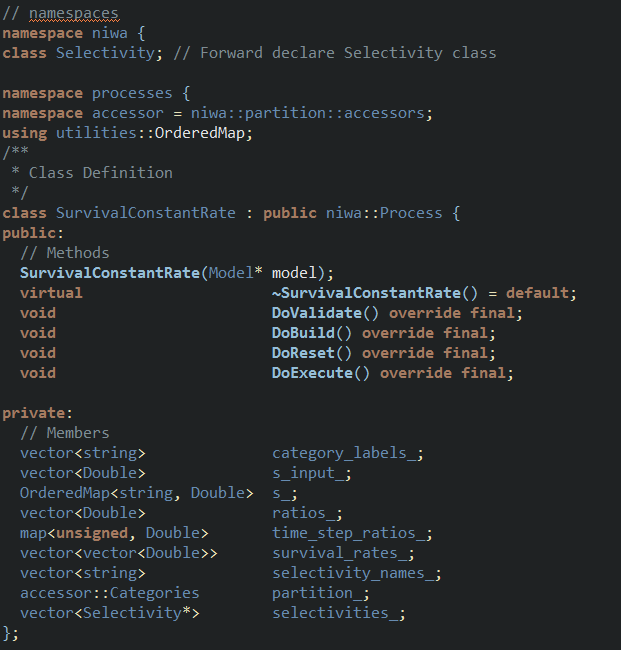
\includegraphics[scale=0.6]{Figures/process_h.png}
	\caption{}\label{fig:process_h}
\end{figure}

We can see that we are implementing \texttt{DoValidate()}, \texttt{DoBuild()}, \texttt{DoExecute()}, \texttt{DoReset()}, which are public functions and we define our variables as private. This idea of structuring classes by public, private and protected is known as encapsulation, and is another important C++ concept. Our variables will be stored in memory for the entire model run so you must make decisions on whether a variable needs to persist for the entire model run or can be temporarily created and destroyed at execution time (Note: the \_ at the end this indicates whether the variable is defined in the \texttt{.h} file or not). 
\\\\
Moving into \texttt{SurvivalConstantRate.cpp}, if we look at the constructor, we can see that this describes input parameters that are supplied by the user, and which variables are estimable. This is applied by the \texttt{RegisterAsEstimable()} function.

\begin{figure}[!ht]
	\centering
	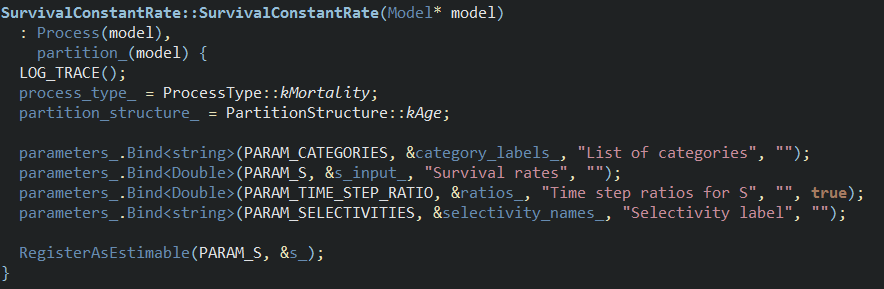
\includegraphics[scale=0.8]{Figures/constructor.png}
	\caption{}\label{fig:constructor}
\end{figure}
When you see keywords that begin with \texttt{PARAM}, for example \texttt{PARAM\_CATEGORIES}, these will be defined in \path{CASAL2\CASAL2\source\English_UK.h}{\color{red}.}

Moving on to the \texttt{DoValidate()} function in Figure~\ref{fig:validate}. The purpose of this function is to validate the user's inputs and expand inputs to allow short hand syntax. You can see the annotation of what is happening in the function. This is considered one of the coding commandments \textbf{Thou shall annotate thy code}.
\begin{figure}[!ht]
	\centering
	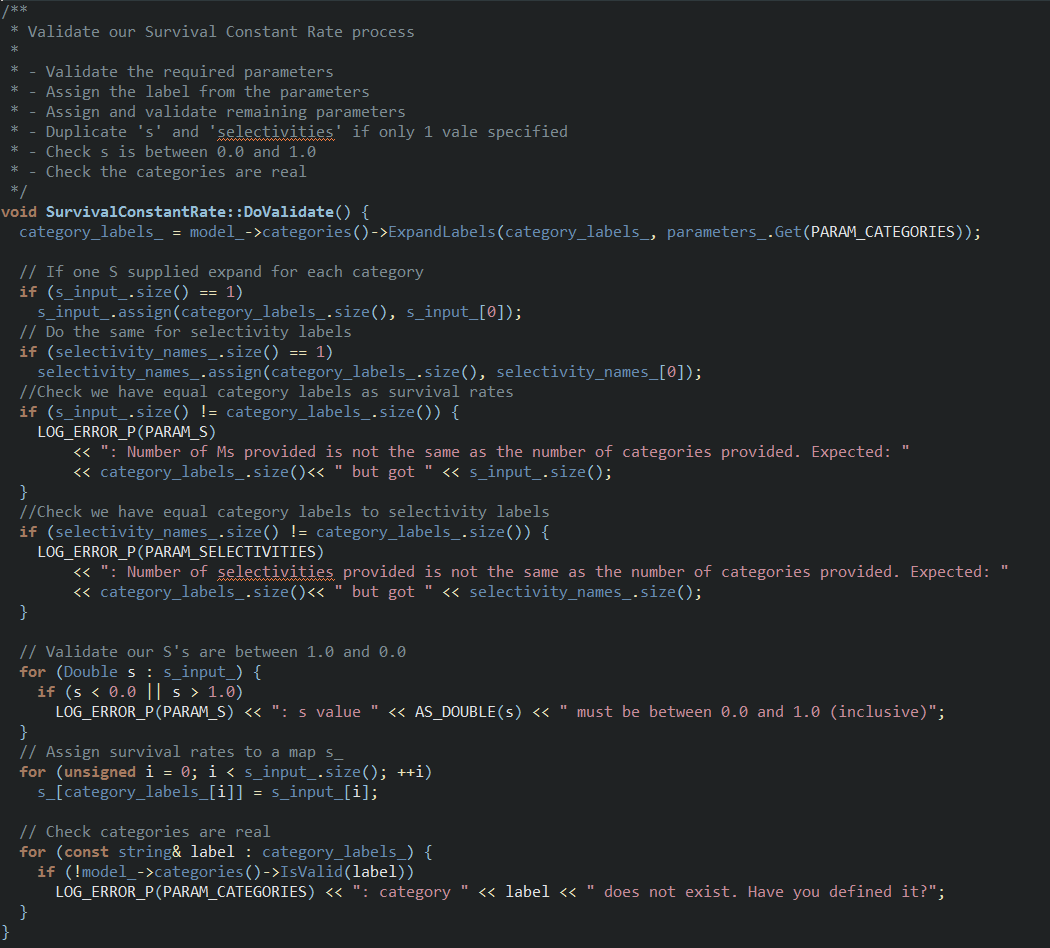
\includegraphics[scale=0.7]{Figures/validate.png}
	\caption{}\label{fig:validate}
\end{figure}

Another nice inclusion to the \CNAME\ source code is it's error checking and messages to the users. The following list is of all the allowable types of errors that \CNAME\ can perform.

\begin{itemize}
	\item \texttt{LOG\_WARNING() << "warning message";} if triggered print the warning message at the end of model run to, warn the user of a change or implication in the model.
	\item \texttt{LOG\_ERROR() << "error message";} After validate and build stop execution and print error message.
	\item \texttt{LOG\_ERROR\_P(PARAM\_KEYWORD) << "error message";} After validate and build stop execution and print error message with location of the parameter \texttt{PARAM\_KEYWORD} in the configuration files.
	\item \texttt{LOG\_FATAL()} if triggered halt execution and print error message.
	\item \texttt{LOG\_FATAL\_P(PARAM\_KEYWORD) << "error message";} If triggered stop execution and print error message with location of the \texttt{PARAM\_KEYWORD} in the configuration files.		
	\item \texttt{LOG\_CODE\_ERROR() << "error message";} if triggered quit \CNAME\ with a message like contact the development team this is a bug in the software.	
\end{itemize}

We encourage you to put these all throughout the validate and build functions, to help users correctly specify models and catch silly input sequences.


Moving on to the \texttt{DoBuild()} function. The purpose of the build function is to create pointers and relationships with other classes that will be required during execution. For example, in this process we will require access to the partition, time step and selectivity classes.

\begin{figure}[!ht]
	\centering
	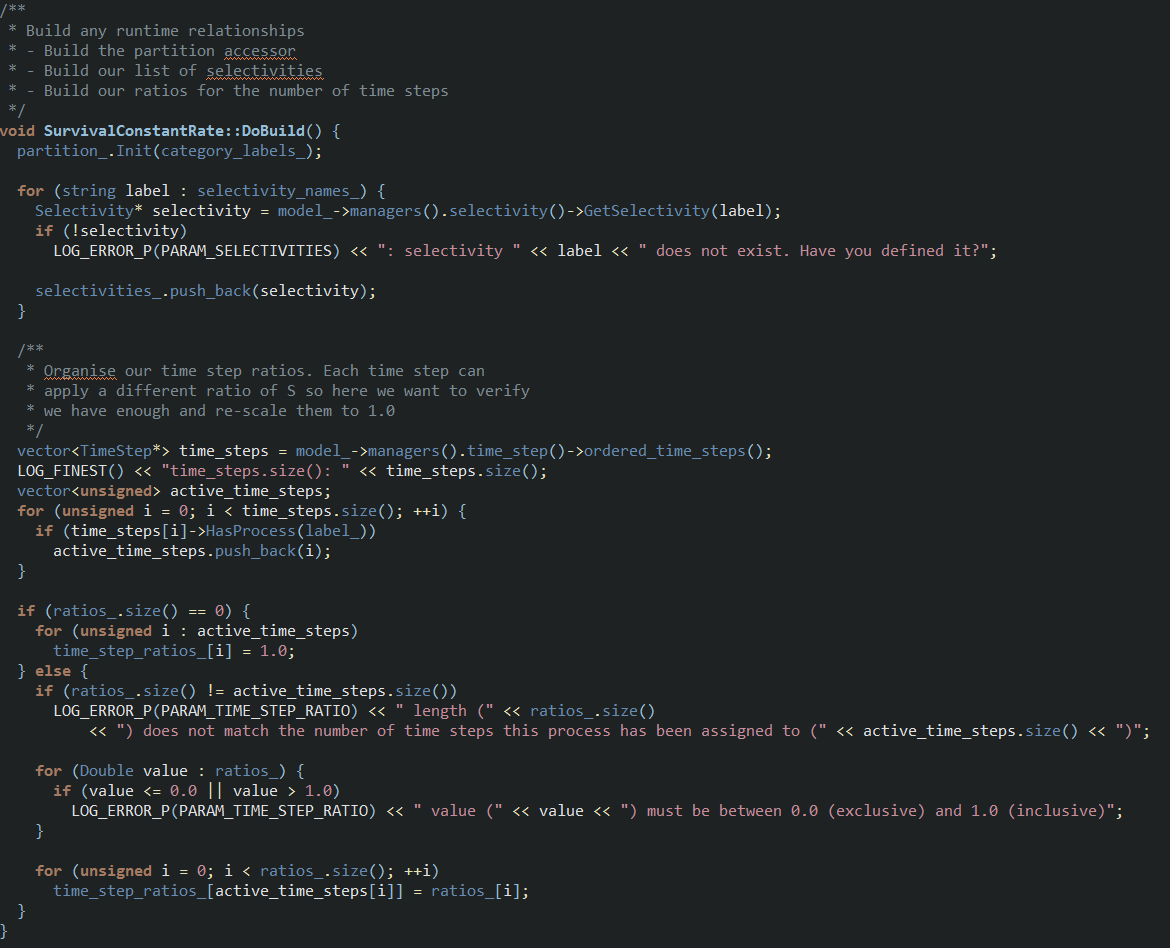
\includegraphics[scale=0.7]{Figures/Build.png}
	\caption{}\label{fig:build}
\end{figure}


Moving on to the \texttt{DoBuild()} function. This is where the action happens and we apply a survival rate to our categories.
\clearpage
\begin{figure}[!ht]
	\centering
	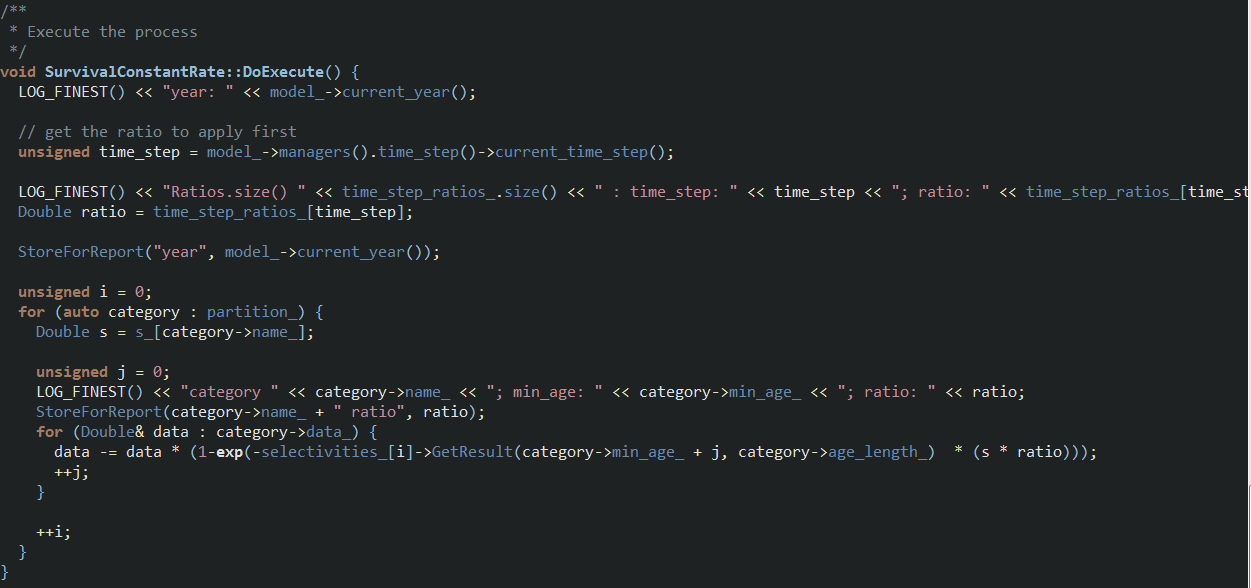
\includegraphics[scale=0.65]{Figures/execute.png}
	\caption{}\label{fig:execute}
\end{figure}

You will notice another set of logging, which is also encouraged to add all throughout the execution process. The levels of logging are described in Section~\ref{subsec:code_practive}

\paragraph*{Adding a unit test}

Still left to do - Samik and Marco to fill in after completing some unit tests.



\section{Adding reports\label{sec:reports}}

This section gives some additional points when adding reports to \CNAME. 

There are two variables that you must define when describing a report class, these are \subcommand{model\_state\_} and \subcommand{run\_mode\_}. We will try and explain what values you should give your report, but another avenue is to look at example report classes. 

The \subcommand{model\_state\_} parameters tells the model when to print the report \subcommand{State::kExecute} will call the \texttt{DoExecute} after each year and \subcommand{State::kIterationComplete} will print the report once the model has run. So obviously if the report prints annual information or doesn't cache information you will want to use \subcommand{State::kExecute} e.g. \subcommand{Partition} else use \subcommand{State::kIterationComplete}. 

\emph{Note:} if you add a new report that has \subcommand{model\_state\_} \subcommand{State::kExecute} you will need to tweak the R-library function \subcommand{extract.mpd()}. At line 50 of the of \texttt{extract.mpd.R} there is the following line of code.   

\begin{lstlisting}[language=R]
multi_year_reports = c("partition", "PartitionBiomass", "PartitionMeanWeight")
\end{lstlisting}

You will need to add the report label type to this vector so that \R\ will process the report correctly.

The other command \subcommand{run\_mode\_} just tells \CNAME\ what run-mode should the report be generated in.

\section{Merging code changes from a branch to the master\label{sec:pull_requests}}

This section describes how to merge changes from a branch to the master repository. See the guidelines in Section~\ref{sec:buildrules} for more information on building \CNAME. 

\emph{Note:} When merging changes, check that the new code doesn't break any of the existing unit-tests or auto-differentiation code. You will need to build using the commands listed below before merging changes.

\begin{enumerate}
	\item \texttt{doBuild archive} this will build all the autodiff librarys.
	\item \texttt{doBuild modelrunner}
	\item Enter the directory  \texttt{BuildSystem\textbackslash Casal2\textbackslash Casal2 - -unittest} to check all the unit-tests pass.
\end{enumerate}

This section differs from Section~\ref{sec:maintain_repo} (where we pulled changes from the master repository into a branch). Here we are merging changes from a branch into the master, which will be incorporated into the master version of \CNAME. From this example we can see from Figure~\ref{fig:fork_merge1} that our branch is 109 commit ahead and 844 commits behind (underlined in blue) that we want to incorporate into the master repository.

To incorporate these changes into the master you need to click on the \enquote{pull request} button. This will prompt a comparison of the changes that you are submitting for inclusion into the master.

\begin{figure}[H]
	\centering
	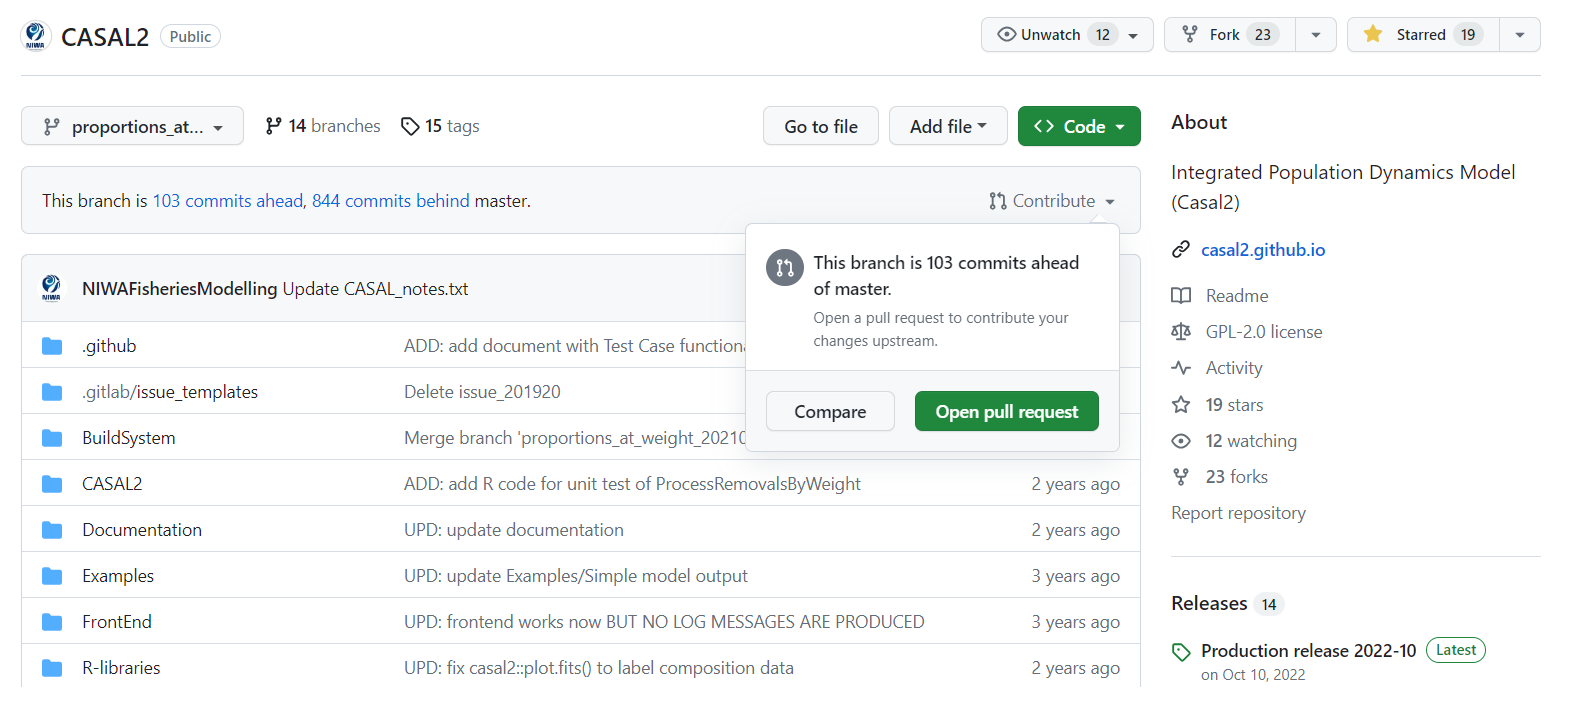
\includegraphics[scale=0.4]{Figures/create_pull_request.png}
	\caption{Example showing differences between a fork and the master in GitHub}\label{fig:fork_merge1}
\end{figure}

We can see that there are ten files changed from three commits. A the top left corner there is a green button with \enquote{create pull request} click that button. This will open a pull request on the master repository as shown in Figure~\ref{fig:fork_merge2}

\begin{figure}[H]
	\centering
	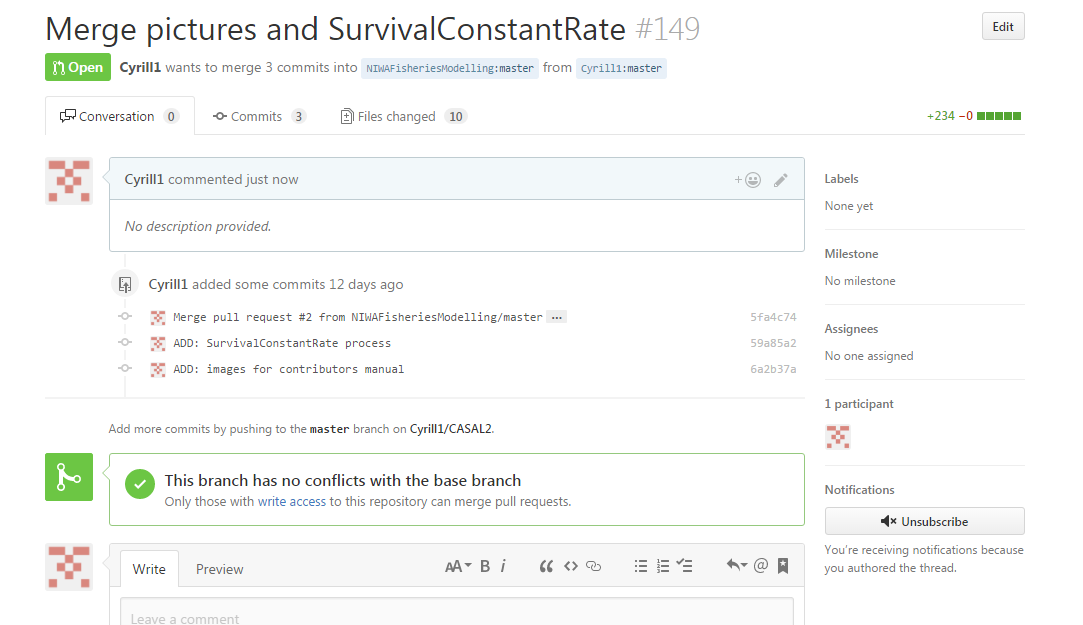
\includegraphics[scale=0.6]{Figures/Pull_request1.png}
	\caption{Example of a pull request in GitHub}\label{fig:fork_merge2}
\end{figure}

This will notify the maintainers of the master repository that a contributor is requesting a merge of the forked code into the master. Maintainers are able to look through the proposed code changed and will discuss the changes with the contributor if they need clarification. But at this point we are just waiting for the maintainers to accept the changes which then get incorporated into \CNAME.


\section{Moderating Code for Maintainers\label{sec:Maintaining}}

This section is for developer responsible for maintaining the GitHub repository, specifically the best way to check a pull request. When we get a pull request the things you want to scrutinize are syntax and optimisation. Why I focus on these is because the automated build system test will tell you if the unit-tests are broken so don't waste your time looking at them. Hopefully who ever is requesting a pull-request has abided by the testing framework and this won't be an issue. \textbf{This section assumes the pull request passes all test's and builds}, please be diplomatic if this is not the truth remembering that we want to encourage collaboration on this project.




\section{Acknowledgements\label{sec:acknowledgements}}


\clearpage{}
% Referencing
\bibliographystyle{plainnat}
\renewcommand{\bibsection}{%
	\section{References}}
\setcitestyle{round,aysep={},yysep={;}%
}
\bibliography{../UserManual/CASAL2}

\end{document}
%End
